% Hlavicka pro protokoly z fyzikalniho praktika.
% Verze pro: LaTeX
% Verze hlavicky: 22. 2. 2007
% Autor: Ustav fyziky kondenzovanych latek
% Ke stazeni: www.physics.muni.cz/ufkl/Vyuka/
% Licence: volne k pouziti, nejlepe k vcasnemu odevzdani protokolu z Vaseho mereni.


\documentclass[czech,11pt,a4paper]{article}
\usepackage[T1]{fontenc}
\usepackage{graphicx, animate}
\usepackage{mathtools}
\usepackage{amssymb}
\usepackage{amsthm}
\usepackage{thmtools}
\usepackage{xcolor}
\usepackage{nameref}
\usepackage{babel}
\usepackage{hyperref}
\usepackage{multicol}
\usepackage[export]{adjustbox}
\usepackage{subcaption}
\usepackage{caption}
\usepackage{multirow}
\usepackage{float}
\usepackage{placeins}
\usepackage{biblatex}
\graphicspath{ {./images/} }




%%% Nemente:
\usepackage[margin=2cm]{geometry}
\newtoks\jmenopraktika \newtoks\jmeno \newtoks\datum
\newtoks\obor \newtoks\skupina \newtoks\rocnik \newtoks\semestr
\newtoks\cisloulohy \newtoks\jmenoulohy
\newtoks\tlak \newtoks\teplota \newtoks\vlhkost
%%% Nemente - konec.


%%%%%%%%%%% Doplnte pozadovane polozky:

\jmenopraktika={Fyzikální praktikum 2}  % nahradte jmenem vaseho predmetu
\jmeno={Teodor Duraković}            % nahradte jmenem mericiho
\datum={9.~prosince 2024}        % nahradte datem mereni ulohy
\obor={F}                     % nahradte zkratkou vami studovaneho oboru
\skupina={Po 14:00}            % nahradte dobou vyuky vasi seminarni skupiny
\rocnik={II}                  % nahradte rocnikem, ve kterem studujete
\semestr={III}                 % nahradte semestrem, ve kterem studujete

\cisloulohy={9}               % nahradte cislem merene ulohy
\jmenoulohy={Polarizace světla} % nahradte jmenem merene ulohy

\tlak={994}                   % nahradte tlakem pri mereni (v hPa)
\teplota={21.6}               % nahradte teplotou pri mereni (ve stupnich Celsia)
\vlhkost={33}               % nahradte vlhkosti vzduchu pri mereni (v %)

%%%%%%%%%%% Konec pozadovanych polozek.


%%%%%%%%%%% Uzitecne balicky:

%%%%%% Zamezeni parchantu:
\widowpenalty 10000 \clubpenalty 10000 \displaywidowpenalty 10000
%%%%%% Parametry pro moznost vsazeni vetsiho poctu obrazku na stranku
\setcounter{topnumber}{3}	  % max. pocet floatu nahore (specifikace t)
\setcounter{bottomnumber}{3}	  % max. pocet floatu dole (specifikace b)
\setcounter{totalnumber}{6}	  % max. pocet floatu na strance celkem
\renewcommand\topfraction{0.9}	  % max podil stranky pro floaty nahore
\renewcommand\bottomfraction{0.9} % max podil stranky pro floaty dole
\renewcommand\textfraction{0.1}	  % min podil stranky, ktery musi obsahovat text
\intextsep=8mm \textfloatsep=8mm  %\intextsep pro ulozeni [h] floatu a \textfloatsep pro [b] or [t]

% Tecky za cisly sekci:
\renewcommand{\thesection}{\arabic{section}.}
\renewcommand{\thesubsection}{\thesection\arabic{subsection}.}
\renewcommand{\thesubsubsection}{\thesubsection\arabic{subsubsection}.}
% Jednopismenna mezera mezi cislem a nazvem kapitoly:
\makeatletter \def\@seccntformat#1{\csname the#1\endcsname\hspace{1ex}} \makeatother


%%%%%%%%%%%%%%%%%%%%%%%%%%%%%%%%%%%%%%%%%%%%%%%%%%%%%%%%%%%%%%%%%%%%%%%%%%%%%%%
%%%%%%%%%%%%%%%%%%%%%%%%%%%%%%%%%%%%%%%%%%%%%%%%%%%%%%%%%%%%%%%%%%%%%%%%%%%%%%%
% Zacatek dokumentu
%%%%%%%%%%%%%%%%%%%%%%%%%%%%%%%%%%%%%%%%%%%%%%%%%%%%%%%%%%%%%%%%%%%%%%%%%%%%%%%
%%%%%%%%%%%%%%%%%%%%%%%%%%%%%%%%%%%%%%%%%%%%%%%%%%%%%%%%%%%%%%%%%%%%%%%%%%%%%%%

\begin{document}
	
	%%%%%%%%%%%%%%%%%%%%%%%%%%%%%%%%%%%%%%%%%%%%%%%%%%%%%%%%%%%%%%%%%%%%%%%%%%%%%%%
	% Nemente:
	%%%%%%%%%%%%%%%%%%%%%%%%%%%%%%%%%%%%%%%%%%%%%%%%%%%%%%%%%%%%%%%%%%%%%%%%%%%%%%%
	\thispagestyle{empty}
	
	{
		\begin{center}
			\sf 
			{\Large Ústav fyzikální elektroniky Přírodovědecké fakulty Masarykovy univerzity} \\
			\bigskip
			{\huge \bfseries FYZIKÁLNÍ PRAKTIKUM} \\
			\bigskip
			{\Large \the\jmenopraktika}
		\end{center}
		
		\bigskip
		
		\sf
		\noindent
		\setlength{\arrayrulewidth}{1pt}
		\begin{tabular*}{\textwidth}{@{\extracolsep{\fill}} l l}
			\large {\bfseries Zpracoval:}  \the\jmeno & \large  {\bfseries Naměřeno:} \the\datum\\[2mm]
			\large  {\bfseries Obor:} \the\obor  \hspace{40mm}  {\bfseries Skupina:} \the\skupina %
			%{\bfseries Ročník:} \the\rocnik \hspace{5mm} {\bfseries Semestr:} \the\semestr  
			&\large {\bfseries Testováno:}\\
			\\
			\hline
		\end{tabular*}
	}
	
	\bigskip
	
	{
		\sf
		\noindent \begin{tabular}{p{3cm} p{0.6\textwidth}}
			\Large  Úloha č. {\bfseries \the\cisloulohy:} \par
			\smallskip
			$T=\the\teplota$~$^\circ$C \par
			$p=\the\tlak$~hPa \par
			$\varphi=\the\vlhkost$~\%
			&\Large \bfseries \the\jmenoulohy  \\[2mm]
		\end{tabular}
	}
	
	\vskip1cm
	
	%%%%%%%%%%%%%%%%%%%%%%%%%%%%%%%%%%%%%%%%%%%%%%%%%%%%%%%%%%%%%%%%%%%%%%%%%%%%%%%
	% konec Nemente.
	%%%%%%%%%%%%%%%%%%%%%%%%%%%%%%%%%%%%%%%%%%%%%%%%%%%%%%%%%%%%%%%%%%%%%%%%%%%%%%%
	
	%%%%%%%%%%%%%%%%%%%%%%%%%%%%%%%%%%%%%%%%%%%%%%%%%%%%%%%%%%%%%%%%%%%%%%%%%%%%%%%
	%%%%%%%%%%%%%%%%%%%%%%%%%%%%%%%%%%%%%%%%%%%%%%%%%%%%%%%%%%%%%%%%%%%%%%%%%%%%%%%
	% Zacatek textu vlastniho protokolu
	%%%%%%%%%%%%%%%%%%%%%%%%%%%%%%%%%%%%%%%%%%%%%%%%%%%%%%%%%%%%%%%%%%%%%%%%%%%%%%%
	%%%%%%%%%%%%%%%%%%%%%%%%%%%%%%%%%%%%%%%%%%%%%%%%%%%%%%%%%%%%%%%%%%%%%%%%%%%%%%%
	
	\begin{multicols}{2}
		\section{Úkoly}
		\begin{enumerate}	
			\item Připravte tři roztoky sacharozy o různé koncentraci $(15 \%, 10 \%, 5 \%)$.
			\item Na dvouhranolovém refraktometru určete index lomu každého z roztoků sacharózy a také čisté vody.
			\item Odečtěte odpovídající koncentraci sacharózy odečtením v refraktometru nebo ji určete podle vztahu 4, grafu 1 nebo z tabulek.
			\item Určete polarimetrem úhel stočení kmitové roviny připravených roztoků. Měření všech kyvet opakujte $5 \times$, vždy ve schématu: nulová poloha - první kyveta - druhá kyveta - třetí kyveta.
			\item Vypočítejte specifickou stáčivost sacharozy a porovnejte ji s tabelovanou hodnotou, kterou najdete např. v tabulce 1
			\item Měření provádějte v monochromatickém světle s vybraným barevným filtrem.
			\item Jeden z polarizátorů nechejte v pevné poloze, druhým otáčejte.
			\item Zaznamenávejte hodnoty fotoproudu na měřidle odpovídající nastaveným úhlům.
			\item Vyneste závislost fotoproudu na úhlu otočení polarizátoru.
			\item Ze vztahu 15 určete stupeň polarizace druhého polarizátoru.
		
		\end{enumerate}
	\section{Teorie}
	\subsection*{Měření indexu lomu a optické stáčivosti roztoku sacharózy}
	Látky rozpuštěné v roztoku ovlivňují mimo jiné jeho optické vlastnosti. Optická měření bývají rychlá, proto se často používají v analýzách roztokù. V této úloze budeme měřit koncentrační závislost indexu lomu a optické stáčivosti roztoku sacharózy.
	
	\subsection*{Závislost indexu lomu roztoku sacharózy na jeho koncentraci}
	\begin{figure}[H]
		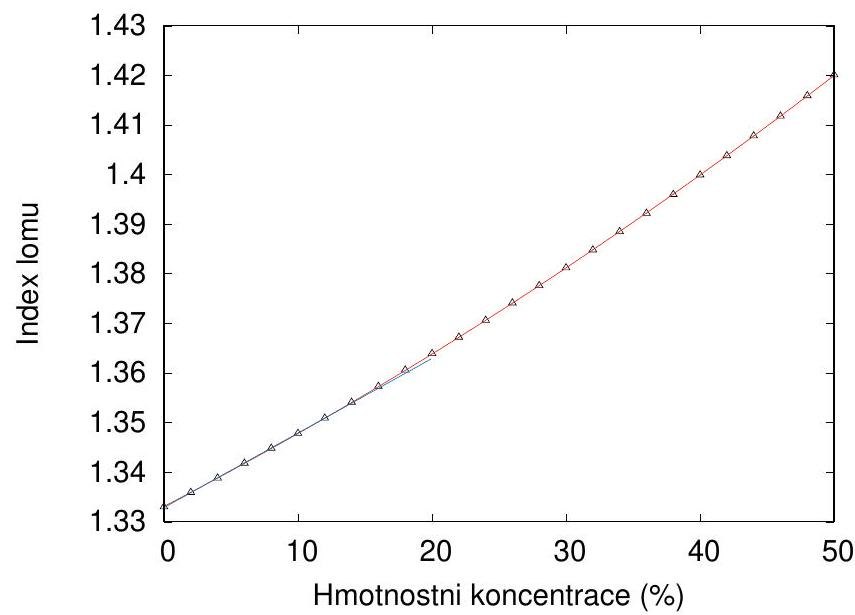
\includegraphics[width=0.95\linewidth,center]{2024_12_10_a013f21445168c71d61fg-1}
		\caption{Závislost indexu lomu roztoku sacharózy. Pro žluté světlo sodíkové výbojky s vlnovou délkou 589 nm. Červenou čarou je vvynesen fit kvadratickou závislostí a modrou lineární aproximace.}
	\end{figure}
	
	
	
	Hmotnostní koncentrace roztoků $c_{m}$ se definuje
	
	
	\begin{equation}
		c_{m}=\frac{m_{\mathrm{sach}}}{m_{\mathrm{raz}}}
	\end{equation}
	
	
	kde $m_{\text {sach }}$ hmotnost rozpuštěné látky a $m_{\text {roz }}$ je hmotnost roztoku. Po vynásobení stem dostaneme hodnotu v procentech. Pro malé koncentrace vodných roztoků se předpokládá, že hustota roztoku se příliš neliší od hustoty vody $1 \mathrm{~g} / \mathrm{cm}^{3}$ a hmotnost roztoku se nahradí jejím objemem
	
	\begin{equation}
		c=\frac{m_{\text {sach }}(\mathrm{g})}{V_{\mathrm{roz}}\left(\mathrm{~cm}^{3}=\mathrm{ml}\right)} 100(\%)
	\end{equation}
	
	
	kde hmotnost rozpuštěné látky $m_{\text {sach }}$ dosazujeme v gramech a objem roztoku $V_{\text {roz }} \mathrm{v}$ kubických centimetrech čili mililitrech. Závislost indexu lomu vodného roztoku sacharózy na jeho koncentraci c je vynesena na obrázku 1. Závislost lze popsat kvadratickou formulí
	
	
{\small 	\begin{equation}
		n(c)=(1,3330 \pm 0,0003)+(0,00140 \pm 0,00003) c+
	\end{equation}
	$(6,7 \pm 0,5) \times 10^{-6} c^{2}$}
	
	kde konstantní člen je roven indexu lomu vody $n_{\text {voda }}$. Pro malé koncentrace do $20 \%$ můžeme s dostatečnou přesností použít i lineární vztah
	
	
	{\small \begin{equation}
		n(c)=(1,3330 \pm 0,0003)+(0,00140 \pm 0,00003) c=
	\end{equation}
	$		=n_{\mathrm{voda}}+(0,00140 \pm 0,00003) c$}
	
	\subsection*{Měření indexu lomu pomocí mezního úhlu}
	Index lomu pevných látek a kapalin lze snadno a s vysokou přesností zjistit měřením mezního úhlu při lomu resp. odrazu na rozhraní dvou prostředí. Máme-li dvě prostředí (viz obr. 2), charakterizovaná indexy lomu $N_{1}$ a $N_{2}\left(N_{1}<N_{2}\right)$ a prochází-li světlo z prostředí o indexu lomu $N_{1}$ do prostředí charakterizovaného indexem lomu $N_{2}$, nastává podle Snellova zákona lom paprsků ke kolmici. V mezním případě, kdy je úhel dopadu roven 90 stupňům (obr. 2, paprsek 2), se šíří světlo ve druhém prostředí pod největším možným úhlem $\beta_{m}$. Tedy do vyšrafované oblasti na obr. 2 nemůže světlo z prvního prostředí po lomu na rozhraní vnikat. Pro mezní úhel $\beta_{m}$ dostáváme podle Snellova zákona
	
	
	\begin{equation}
		\sin \beta_{m}=\frac{N_{1}}{N_{2}}
	\end{equation}
	
	
	Na principu měření mezního úhlu jsou konstruovány refraktometry, kterými lze určit index lomu rychle a s použitím malého množství měřené látky (kapaliny).
	
	\subsection*{Dvouhranolový refraktometr}
	Základní částí přístroje jsou dva hranoly $H_{1}$ a $H_{2}$, zhotovené ze skla s vysokým indexem lomu (obr. 3). Měřící hranol $H_{1}$ má stěny $A C$ a $B C$ vyleštěny, strana $A B$ je zmatovaná. Osvětlovací\\
	\begin{figure}[H]
			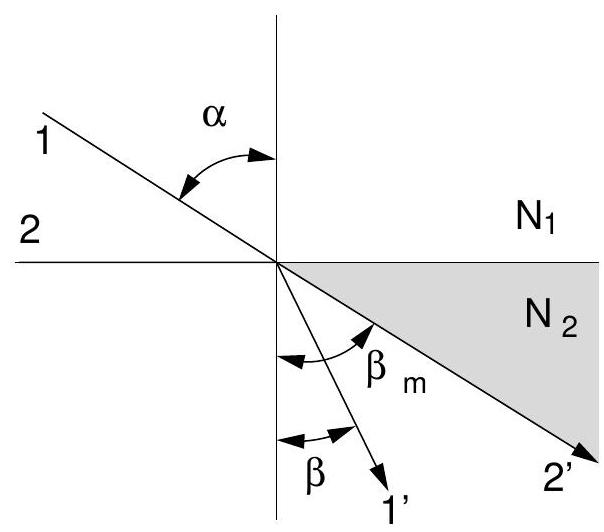
\includegraphics[width=0.95\linewidth,center]{2024_12_10_a013f21445168c71d61fg-2}
			\caption{Lom světelného paprsku na rozhraní dvou prostředí pro případ $N_{2}>N_{1}$. Dále je vyznačen mezní úhel $\beta_{m}$ a žlutě oblast, do níž světlo může procházet. Žádné světlo se neláme do šedě vyznačené oblasti.\\
				hranol $H_{2}$ má naopak zmatovanou stěnu $E D$. Měřený objekt se umistuje na plochu $A C$ měřícího hranolu. Je-li měřen index lomu kapaliny, jsou oba hranoly k sobě přiklopeny a mezi ně se vpraví malé množství kapaliny. Chceme-li měřit index lomu pevné látky, musí mít vzorek alespoň jednu plochu rovinnou a dobře vyleštěnou. Vzorek přiložíme touto plochou na stěnu $A C$, na kterou je třeba před měřřením nanést malé množství kapaliny s indexem lomu vyšším než má měřená látka (obvykle 1-bromnaftalem, $n=1,658$ )}
	\end{figure}
	
	
	
	\begin{figure}[H]
		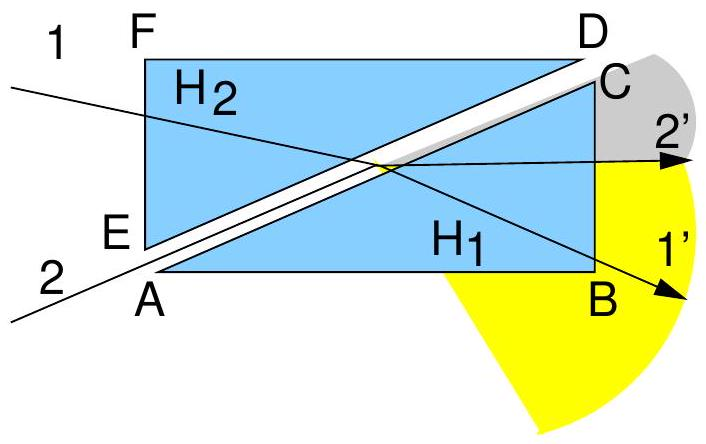
\includegraphics[width=0.95\linewidth,center]{2024_12_10_a013f21445168c71d61fg-3}
	
	\caption{Optický princip dvojhranolového refraktometru. Při lomu z měřeného matriálu umístěného mezi hranoly na stěně $A C$ hranolu $H_{1}$ se veškeré světlo láme do žlutě vyznačené výseče, šedá výseč je temná. Směr mezního paprsku 2', který oděluje světlou a temnou oblast, je dán indexem lomu měřeného materiálu umístěného mezi hranoly podle vztahu (10.5). být menší než index lomu hranolu $H_{1}$, aby se světlo lámalo ke kolmici.}
	\end{figure}
	
	Při měření na průchod vstupuje světlo plochou $E F$ do osvětlovacího hranolu, na ploše $E D$ se rozptýlí a vchází do měřené látky. Po lomu vychází stěnou $B C$. Tato plocha je pozorována dalekohledem. Při měření v monochromatickém světle je mezi oběma částmi zorného pole ostré rozhraní. Při měření na odraz vstupuje světlo plochou $A B$ do hranolu $H_{1}$ a po odrazu opět vychází plochou $B C$.
	
	Je-li měření prováděno v bílém světle, je rozhraní v zorném poli dalekohledu zbarveno. Aby se tato obtíz odstranila, je dvojhranolový refraktometr vybaven kompenzátorem, což jsou dva Amiciovy hranoly. Činnost kompenzátoru spočívá v tom, že se do optické soustavy přístroje zařadí nový hranol, jehož disperze je až na znaménko rovna disperzi měřící soustavy.
	
	S měřícím hranolem je pevně spojena stupnice kalibrovaná v hodnotách indexu lomu. Odečítá se na ní pomocí lupy umístěné vedle okuláru dalekohledu. Měření na tomto přístroji lze provádět bud' v monochromatickém světle sodíkové výbojky (vlnová délka $589,3 \mathrm{~nm}$ ) nebo ve světle bílém. Refraktometr má rovněž vedle stupnice indexu lomu dodatečnou stupnici pro měření koncentrace roztoku sacharózy.
	
	Postup měření:
	
	\begin{enumerate}
		\item Měření provádějte pro všechny roztoky sacharózy a také pro destilovanou nebo deionizovanou vodu. Odečtené hodnoty indexu lomu a koncentrace sachrózy pro čistou vodu se použijí pro kalibraci refraktometru, tj. jako počátek stupnice pro určení koncentrace sacharózy v roztocích.
		\item Na měřící hranol nanést malé množství měřené kapaliny a přiklopit osvětlovací hranol.
		\item Šroubem na pravé straně přístroje otáčet hranolem tak dlouho, až se v zorném poli dalekohledu objeví rozhraní světlo-tma. Toto rozhraní otáčením šroubu nastavit do průsečíku nitkového kříže v zorném poli dalekohledu.
		\item Na stupnici vpravo lupou odečíst hodnotu indexu lomu měřené kapaliny a koncentraci roztoku sacharózy.\\
	
	\end{enumerate}
	\begin{figure}[H]
			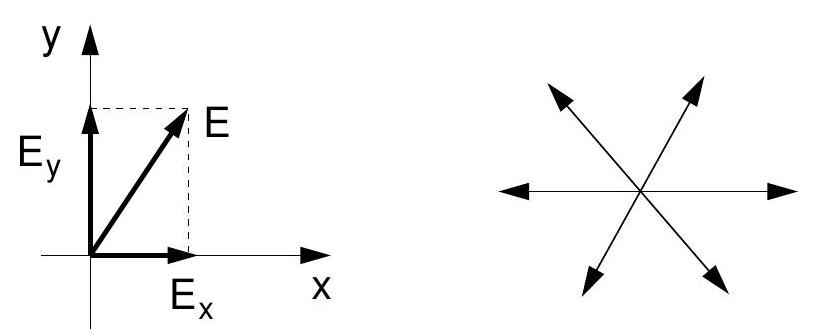
\includegraphics[width=0.95\linewidth,center]{2024_12_10_a013f21445168c71d61fg-4}
			\caption{Polarizace denního svĕtla.}
	\end{figure}
	
	\subsection*{Polarizace světla}
	Světlo je příčné vlnění elekromagnetického pole. Pro popis svĕtelných jevů plně postačí se zaměřit na chování periodicky proměnného vektoru elektrického pole $\vec{E}$. Tento vektor je vždy kolmý ke směru šíření paprsku. Je-li směr vektoru $\vec{E}$ ve všech bodech paprsku v čase stálý, hovoříme o lineárně polarizovaném světle a rovina, v níž se kmity dějí, se nazývá kmitová rovina nebo rovina polarizace. Lineárně polarizované světlo můžeme dostat lomem nebo odrazem.
	
	Je vhodné rozložit vektor elektrického pole $\vec{E}$ do dvou navzájem kolmých směrů a vyjádřit ho ve složkách $E_{x}$ a $E_{y}$ (obr. 4, přičemž se světelný paprsek šíří kolmo k rovině obrázku). Je-li fázový posuv $\delta$ mezi tĕmito složkami stálý a je-li zároveň roven nule, dostávame lineárně polarizované světlo. V případě, že $\delta=\pi / 2$ a navíc platí $E_{x}=E_{y}$ opisuje koncový bod vektoru $\vec{E}$ kružnici a dostáváme kruhově polarizované světlo; v obecném případě, kdy $0<\delta<\pi / 2$ jde o elipticky polarizované vlnění.
	
	\subsection*{Optická aktivita látek}
	Látky jsou opticky aktivní, mají-li schopnost stáčet rovinu lineárně polarizovaného světla. Tuto vlastnost mají jak některé látky pevné tak i některé roztoky obsahující v molekule např. asymetricky umístěný uhlík (vodný roztok sacharozy). Podle směru stočení kmitové roviny se opticky aktívní látky dělí na pravo- a levotočivé vzhledem k pozorovateli hledícímu proti směru šíření světla. Biot stanovil empirický vztah pro úhel stočení kmitové roviny po průchodu aktivní látkou,
	
	
	\begin{equation}
		\alpha=[\alpha] d
	\end{equation}
	
	
	kde $[\alpha]$ je specifická stáčivost zkoumané látky a $d$ je tloušťka této látky. Veličina $[\alpha]$ závisí na teplotě a vlnové délce světla. Jde-li o roztoky, pak
	
	\begin{equation}
		\alpha=[\alpha] c d
	\end{equation}
	
	
	kde $c$ označuje koncentraci opticky aktivní látky. Specifickou stáčivost roztoku lze stanovit ze vztahu (10.7) polarimetrem:
	
	
	\begin{equation}
		[\alpha]=\frac{100 \alpha}{d q}
	\end{equation}
	kde $q$ je počet gramů látky ve $100 \mathrm{~cm}^{3}$ roztoku.
	Tabulka 1: Specifická stáčivost vybraných látek.
	
	\begin{center}
		\begin{tabular}{|l|r|}
			\hline
			látka & s. stáčivost $\left({ }^{\circ} \mathrm{cm}^{3} / \mathrm{g} . \mathrm{dm}\right)$ \\
			\hline
			Sacharóza & $+66,53$ \\
			Fruktóza & $-93,78$ \\
			Dextróza & $+52,74$ \\
			\hline
		\end{tabular}
	\end{center}
	
	\begin{figure}[H]
		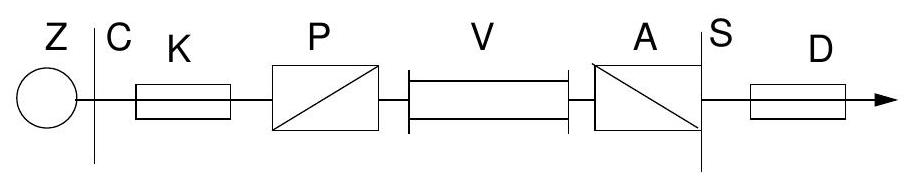
\includegraphics[width=0.95\linewidth,center]{2024_12_10_a013f21445168c71d61fg-5}
		\caption{Polarimetr}
	\end{figure}
	

	
	\subsection*{Polarimetr}
	Polarimetr slouží k měření úhlu stočení roviny polarizace studovanou látkou (kapalnou, pevnou či plynnou). Polarimetr je znázorněn na obr. 5. Světlo z monochromatického zdroje (Z) je kolimátorem (K) zpracováno na rovnoběžný svazek paprsků. Průchodem přes polarizátor (P) se vlnění lineárně polarizuje a bud’ prochází přes měřený vzorek (V) nebo jde přímo na analyzátor (A), kterým lze otáčet kolem optické osy přístroje. Výsledná intenzita prošlého světla se pozoruje dalekohledem (D). Polarizátor a analyzátor jsou zpravidla realizovány pomocí speciálních hranolů z opticky anizotropních krystalů. Zkřížíme-li kmitové roviny polarizátoru a analyzátoru, bude intenzita osvětlení zorného pole minimální. Naše oči pozorují minimum osvětlení dosti nepřesně a nespolehlivě, naopak jsou citlivé na kontrast v osvětlení dvou sousedních ploch. Tohoto poznatku se využívá při konstrukci tzv. polostínového zařízení analyzátoru, kde se snažíme dosáhnout otáčením analyzátoru takového stavu, při kterém jsou obě poloviny zorného pole osvětleny stejně (málo). Úhel stočení analyzátoru vůči polarizátoru se měří na stupnici (S).
	
	\section*{Měření}
	Připravíme asi $25 \mathrm{~cm}^{3} 15 \%$ roztoku sacharozy a nalijeme do kyvety. Zbytek roztoku zředíme tak, abychom získali $10 \%$ roztok sacharozy a znovu odlejeme do druhé kyvety. Postup ještě jednou zopakujeme tak, aby ve třetí kyvetě byl $5 \%$ roztok sacharozy.
	
	Zapneme výbojku před polarimetrem. Otáčením analyzátoru nastavíme polostín a odečteme na stupnici nulovou polohu (pozor na správnou stupnici). Kyvetu s roztokem vložíme do přístroje a opět najdeme polostín a na stupnici odečteme úhel stočení. Ze vztahu (8) určíme specifickou stáčivost, měření opakujeme alespoň $5 \times$.
	

	
	\section*{Malusův zákon, měření polarizační schopnosti reálných polaroidů}
	\section*{Úvod}
	Zdroje světla si lze představit jako soubor velkého množství vzájemně nezávislých zdrojů elektromagnetického záření (atomy,molekuly). Světlo vyzařované např. jedním atomem je lineárně\\
	polarizované tzn. že vektor intenzity elektrického pole $\vec{E}$ se v čase mění v přesně definované rovině - rovině kmitové. V daném okamžiku se ale ve směru šířícího se paprsku světla šíří energie vyzařovaná mnoha elementárními zdroji. V tomto případě jsou v postupující vlně zastoupeny všechny možné kmitové roviny, hovoříme o přirozeném světle.
	
	Z přirozeného světla můžeme dostat lineárně polarizovanou vlnu pomocí polarizačních přístrojů - polarizátorů. Při odrazu světla na dielektrickém rozhraní závisí odrazivost různě polarizovaných složek na úhlu dopadu podle Fresnelových vztahů. Tento jev je studován v úloze 7. Plně polarizované světlo lze získat při odrazu pod Brewsterovým úhlem. Také světlo po lomu na rozhraní je částečně polarizováno. Klasické polarizátory (Nikolův hranol) využívají dvojlomu v některých krystalech, kdy index lomu závisí na polarizaci. Různě polarizované složky se pak šíří pod různými směry a jednu z nich lze eliminovat při totálním odrazu na jiné stěně hranolu. V současné době se nejvíce používají polarizační fólie (polaroidy) tvořené uspořádanými polymerními vlákny. Propustnost folie je závislá na polarizaci světla. Při vhodné volbě materiálu a tloušťky lze připravit polarizační folie s vysokou účinností.
	
	\section*{Malusův zákon}
	Na obrázku 6 označuje P polarizátor, A analyzátor, $I_{0}$ je intenzita přirozeného světla dopadajícího na polarizátor, $I_{0}^{\prime}$ je intenzita světla po průchodu polarizátorem. Dále je $I$ intenzita svazku, který prošel analyzátorem A a $\alpha$ je úhel mezi kmitovými rovinami vektoru $\vec{E}$ před a po průchodu analyzátorem. Označíme-li amplitudu vektoru $\vec{E}$ před průchodem analyzátorem $a_{0}$ a po průchodu $a$, pak podle předchozího obrázku platí
	
	
	\begin{equation}
		a=a_{0} \cos \alpha
	\end{equation}
	
	
	Intenzita světla je úměrná druhé mocnině amplitudy, tedy intenzita prošlého světla analyzátorem je dána vztahem
	
	\begin{equation}
		I=I_{0}^{\prime} \cos ^{2} \alpha
	\end{equation}
	
	
	což je matematický zápis Malusova zákona. V případě nedokonalých polarizátorů bude část světla pronikat i při zkřížených polarizátorech. Malusův zákon pak můžeme upravit
	
	\begin{equation}
		I(\alpha)=I_{\min }+\left(I_{\max }-I_{\min }\right) \cos ^{2} \alpha
	\end{equation}
	
	
	\begin{figure}[H]
		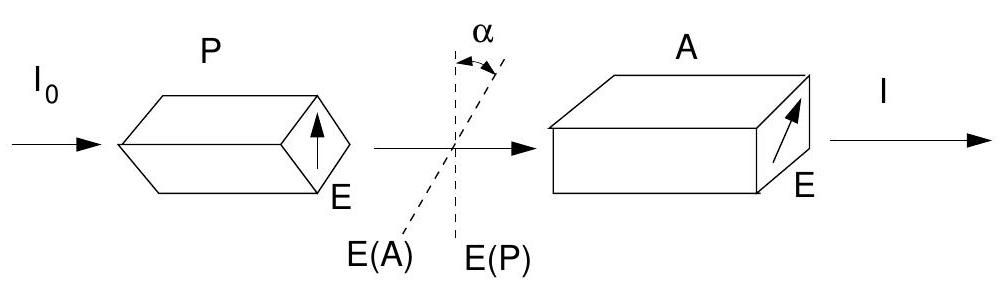
\includegraphics[width=0.95\linewidth,center]{2024_12_10_a013f21445168c71d61fg-6}
		\caption{Schéma Malusova pokusu.}
	\end{figure}
	
	
	
	\section*{Ověření platnosti Malusova zákona}
	Využijeme uspořádání podle obr. 7 se dvěma polarizátory (Nikolovým hranolem a polarizační fólií) a světelný zdroj umístíme tak, aby světlo procházelo oběma polarizátory. Platnost Malusova zákona ověříme tak, že jeden z polarizátorů necháme v libovolné, ale stále stejné poloze a druhým budeme otáčet s pevným krokem v rozsahu $0^{\circ}$ až $360^{\circ}$. Závislost fotoproudu na úhlu stočení obou polarizátorů by měla odpovídat závislosti dle vztahu 11. Tuto závislost můžeme ještě dále využít ke stanovení stupně polarizace světla. Částečně polarizované světlo si lze představit\\
	složeno z části polarizované (intenzita $I_{p}$ ) a části nepolarizované $\left(I_{n}\right)$. Stupeň polarizace $V$ částečně polarizovaného světla je dán vztahem
	
	
	\begin{equation}
		V=\frac{I_{p}}{I_{p}+I_{n}}
	\end{equation}
	
	
	\begin{figure}[H]
		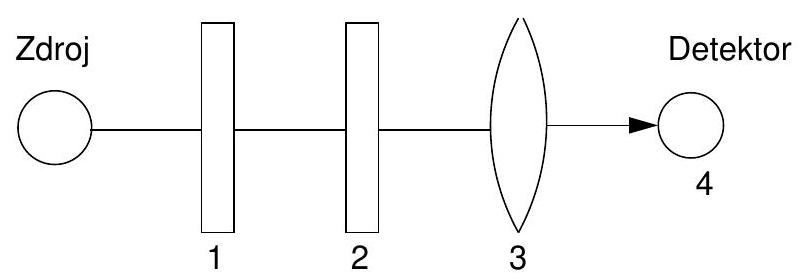
\includegraphics[width=0.95\linewidth,center]{2024_12_10_a013f21445168c71d61fg-7}
		\caption{Uspořádání pro ověření Malusova zákona. 1 - první polarizátor, 2 - druhý polarizátor, 3 - fokusační čočka, 4 - detektor.}
	\end{figure}
	
	
	Mějme dva polarizátory z nichž první je nedokonalý (s nízkým stupněm polarizace) a druhý téměř dokonalý. Předpokládejme, že propustnost druhého polarizátoru pro světlo polarizované v polarizační rovině polarizátoru je rovna 1 a pro světlo polarizované kolmo k jeho polarizační rovině rovna 0 . Testujeme stupeň polarizace prvního polarizátoru. Po průchodu polarizátorem č. 1 jsou intenzity polarizovaného světla $I_{p}^{(1)}$ a $I_{n}^{(1)}$. Jsou-li kmitové roviny obou polarizátorů rovnoběžné, dostaneme po průchodu světla oběma polarizátory intenzitu
	
	\begin{equation}
		I_{\max }=I_{p}^{(1)}+\frac{I_{n}^{(1)}}{2}
	\end{equation}
	
	
	protože linárně polarizovaná složka projde i druhým polarizátorem, ale z nepolarizované složky jen jedna polovina. Naopak, jsou-li kmitové roviny navzájem kolmé, pak projde přes druhý polarizátor pouze polovina z nepolarizované složky
	
	
	\begin{equation}
		I_{\min }=\frac{I_{n}^{(1)}}{2}
	\end{equation}
	
	
	Dosadíme-li $I_{p}^{(1)}$ a $I_{n}^{(1)}$ do vztahu 12 , dostaneme pro stupeň polarizace vztah
	
	\begin{equation}
		V=\frac{I_{\max }-I_{\min }}{I_{\max }+I_{\min }}
	\end{equation}
	
	
	Stupeň polarizace tedy určíme ze závislosti fotoproudu na úhlu stočení polarizátoru.
	
	
	
	
		\section{Měření}
		Namícháme roztoky sacharózy o koncentraci 5, 10, 15 \%. Z měření na dvouhranolovém refraktometru nejdříve musíme stanovit hodnoty při nulové koncentraci u našeho roztoku, získáváme:
		
		\begin{tabular}{l|l}
			c[\%] & n \\	\hline		
			-0.50 $\pm 0.09 $ & 1.3321 $\pm 0.00017$ \\
			-0.50 $\pm 0.09 $& 1.3321 $\pm 0.00017$\\
			-0.45 $\pm 0.09 $& 1.3322 $\pm 0.00017$\\ \hline
			-0.48 $\pm$0.09 & 1.33213 $\pm$0.00017 \\
			
		\end{tabular}\\
		Pro jednotlivé koncentrace tudíž získáme:
		
		\begin{tabular}{l|rr}
			$c_0 [\%]$ & c [\%]               & n                       \\ \hline
			15  & 15.05$\pm$0.12  & 1.35500 $\pm $ 0.00017 \\
			10  & 9.95$\pm$0.12   & 1.34700 $\pm$ 0.00017  \\
			5   & 4.99$\pm$ 0.12 & 1.33690 $\pm$ 0.00017  \\
			0   & 0               & 1.33213 $\pm$ 0.00017 
		\end{tabular}
		
		A ze stáčivosti formulí (8) určíme hodnotu specifické stáčivosti (Hodnoty jsou již vztaženy k upravené nulové hodnotě)
		
	\begin{center}
			{\tiny \begin{tabular}{lllll}
		& $\alpha _{15}$  & $\alpha _{10}$   & $\alpha _{5}$    & $\alpha _{0}$  \\
		& 10.35+/-0.12  & 6.60+/-0.12    & 3.30+/-0.12    & -0.10+/-0.12 \\
		& 10.25+/-0.12  & 6.80+/-0.12    & 3.30+/-0.12    & 0.10+/-0.12  \\
		& 10.30+/-0.12  & 6.75+/-0.12    & 3.30+/-0.12    & -0.00+/-0.12 \\ \hline
		$\overline{\alpha}$& 10.30+/-0.12  & 6.72+/-0.12    & 3.30+/-0.12    & 0.0+/-0      \\ \hline \hline
		$ [\alpha] $ & 68,74 $\pm$ 1 & 67.5 $\pm$ 1.5 & 66.1 $\pm$ 2.9 &             
		\end{tabular}}
	
	\begin{equation}
		[\alpha] = 67.4 \pm 1.5 \,\mathrm{cm^3 g^{-1} dm^{-1} }
	\end{equation}
	
	\subsection{Malusův zákon}
	Z měření bez a s monochromatickým filtrem (f684: 689nm) získáváme: \\
	\begin{tabular}{l|rr}
		$\varphi [^\circ]$ & $I_0 \,\rm[mA]$ & $I\,\rm [\mu A]$ \\
		0               & 1.23            & 1.79              \\
		20              & 1.302           & 2.67              \\
		40              & 1.386           & 3.58              \\
		60              & 1.45            & 4.06              \\
		80              & 1.42            & 3.9               \\
		100             & 1.362           & 3.18              \\
		120             & 1.274           & 2.26              \\
		140             & 1.207           & 1.53              \\
		160             & 1.188           & 1.34              \\
		180             & 1.222           & 1.77              \\
		200             & 1.305           & 2.64              \\
		220             & 1.37            & 3.51              \\
		240             & 1.436           & 3.97              \\
		260             & 1.407           & 3.8               \\
		280             & 1.355           & 3.12              \\
		300             & 1.274           & 2.2               \\
		320             & 1.203           & 1.46              \\
		340             & 1.19            & 1.32             
	\end{tabular}
	\begin{figure}[H]
		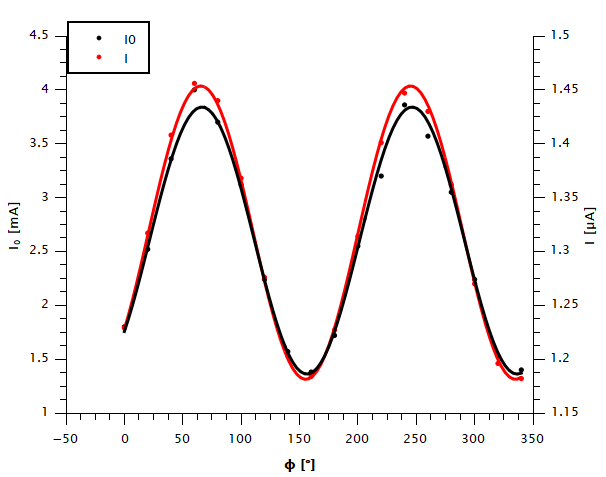
\includegraphics[width = 0.95\linewidth, center]{zavislost}
		\caption{Závislost fotoproudu na úhlu otočení polarizátoru}
	\end{figure}
	Pro bílé světlo platí: $I_{max} = 4.0361 \pm 0.003, I_{min} = 1.3124 \pm 0.003 \,\mathrm{mA}$
	Pro filtrované světlo: $I_{max} = 1.4342 \pm 0.03, I_{min} = 1.1861  \pm 0.03 \,\mathrm{\mu A}$
	
	Proto $V_0 = 0.5092 \pm 0.0009, \, V = 0.095 \pm 0.016.$
		
	\end{center}
		\section{Závěr}
		Podařilo se nám splnit veškeré zadané úkoly a získat hodnoty hledaných veličin. Finální hodnota - s. stáčivý úhel - se od hodnoty v tab. 1 odlišuje v rámci vlastní nejistoty, což je poměrně pěkný výsledek. 
		
	
		

		
		
		
		
		
		% Nakonec nezapomeňte projet text programem vlna nebo vlnka, např.
		% 	vlna -m -l -n mojeuloha.tex
		% nebo zkontrolovat a opravit jednopísmenné předložky na koncích řádků ručně.
	\end{multicols}
\end{document}
